\documentclass[twoside,openright,final]{bhamthesis}
\usepackage[utf8]{inputenc}
\usepackage{amssymb}
\usepackage{amsmath}
\usepackage{listings}
\usepackage{geometry}
\usepackage{indentfirst}
\usepackage{graphicx}
\graphicspath{ {images/} }
\usepackage{enumerate,letltxmacro}
\LetLtxMacro\itemold\item
\renewcommand{\item}{\itemindent0.5cm\itemold}

\pagestyle{plain}

\setlength{\oddsidemargin}{1cm} % 2cm margin on the left for odd pages
\setlength{\evensidemargin}{0cm} % 2cm margin on the right for even pages

\title{Certified Parsing of Regular Expressions in Agda}
\department{Computer Science}
\degree{BSc. Computer Science}
\author{Wai Tak, Cheung}
\studentid{1465388}
\supervisor{Dr. Martín Escardó}

\begin{document}
\maketitle

\abstract
\par Blah blah blah. Blah blah blah. Blah blah blah. Blah blah blah. Blah
blah blah. Blah blah blah. Blah blah blah. Blah blah blah.
Blah blah blah. Blah blah blah. Blah blah blah. Blah blah blah. Blah
blah blah.
Blah blah blah. Blah blah blah. Blah blah blah. Blah blah blah.
Blah blah blah. Blah blah blah. Blah blah blah. Blah blah blah. \\ \\
Keywords: language, regular expression, finite automata, agda,
thompson's construction, powerset construction, proofs

\acknowledgments
\par Blah blah blah. Blah blah blah. Blah blah blah. Blah blah blah. Blah
blah blah. Blah blah blah. Blah blah blah.
Blah blah blah. Blah blah blah. Blah blah blah.
Blah blah blah. Blah blah blah. Blah blah blah. Blah blah blah. Blah
blah blah. Blah blah blah. Blah blah blah.
Blah blah blah. Blah blah blah. Blah blah blah. Blah blah blah. Blah
blah blah. Blah blah blah.
Blah blah blah. Blah blah blah. Blah blah blah. Blah blah blah. Blah
blah blah.

\repository
\vspace{7cm}
\begin{center}
  All software for this project can be found at \\
  https://codex.cs.bham.ac.uk/svn/projects/2015/wtc488/
\end{center}

\newpage
\tableofcontents
\newpage

\section{List of Abbreviations}
\begin{tabular}{ll}
  \textbf{\(\epsilon\)-NFA} & Non-deterministic finite automata with
                              \(\epsilon\)-transition \\
  \textbf{NFA} & Non-deterministic finite automata \\
  \textbf{DFA} & Deterministic finite automata 
\end{tabular}

\section{Introduction}
This work aims to formalise the parts in Formal Language Theory and
Automata Theory that are related to regular languages and finite automata
using Agda. The project is separated into three parts: 1) translating
regular expressions to NFA and DFA, 2) proving the correctness of
the translation and 3) formalising the Myhill-Nerode Theorem.

\par (Here will be a paragraph emphasising the importance of
parsing/automata)

\par The next section will be an introduction on proof assistance and
a review on related reseach topic. After that, the thrid section will
be a detail description of our approach followed by the
evaluation. Finally, we will draw the conclusions. 


\section{Literature Review}
\subsection{Constructive Logic and Constructive Mathematics}
Blah
\subsection{Curry-Howard Isomorphism}
Relations between programs and proofs.
\subsection{Intuitionistic Type Theory}
Blah
\subsection{Agda}
Brief introduction on how agda works as a proof assistant, and how to
write proofs in agda.
\subsection{Related Work}
The matrix representation.


\section{Formalisation in Type Theory}
Let us recall the three objectives of the project: 1) translating
regular expressions to NFA and DFA, 2) proving the correctness of the translation 
and 3) formalising the Myhill-Nerode Theorem. In part 1), we first followed Thompson's
construction algorithm to build an \(\epsilon\)-NFA from a
regular expression. Then we removed all its \(\epsilon\)-transitions by computing the
\(\epsilon\)-closure for each state. Finally, we used powerset
construction to determinise the automata. (Minimize?) 

\par In this section, we will walk through the agda formalisation of
each of these steps together with their correctness proofs. However,
before we can go into these steps, we will have to define a
representation of subset as it is one of the fundamental elements in
Language Theory.

\subsection{Subsets and Decidable Subsets}
\paragraph{Agda} Please refers to Subset.agda and Subset/DecidableSubset.agda

\paragraph{Definition 1.1} Suppose \(A\) is a set, in type theory, we represent its subsets as a unary function on
\(A\), i.e. \(Subset\ A = A \to Set\). \\

\par When declaring a subset, we can write \(SubA =
\lambda\ a \to\ ?\) in Agda, the \(?\) here corresponds to the
condition for an element of \(A\) to be included in \(SubA\). This construction is
very similar to set comprehension. For example, the subset 
\(\{a\ | \ a \in A,\ P(a)\}\) corresponds to \(\lambda\ a \to P\
a\). As we mentioned before, a function in the form of \(A \to
Set\) is also a predicate of \(A\). Therefore, Subset is also a unary
predicate of \(A\). Thus, the decidibilty of Subset will remain
unknown until it is proved. 

\paragraph{Definition 1.2} The other representation of subset is \(DecSubset\ A = A \to
Bool\). Unlike \(Subset\), its decidability is ensured by its
definition. \\

\par The two definitions have different purposes. \(Subset\) was used to represent \(Language\) because not every
language is decidable. For other parts in the project 
such as the subset of states of an automata, \(DecSubset\) was used
as the decidability was assumed in the definition. The two definitions
are defined in Subset.agda and Subset/DecidableSubset.agda
respectively as stated at the top, operatiors such as membership (\(\in\)), subset
(\(\subseteq\)), superset (\(\supseteq\)) and eqaulity (\(=\)) can
also be found in the two files. 

\par Now, by using the subset representation, we can define languages, regular expressions and finite
autotmata. Their formalisation in this project followed tightly to the
definition from Aho, A. and Ullman, J. (1972). 

\subsection{Languages}
\paragraph{Agda} Please refers to Language.agda \\

\par Suppose we have a set of alphabet \(\Sigma\). In type theory, it will be a data type,
i.e. \(\Sigma : Set\). Notice that the decidable equality of
\(\Sigma\) is assumed, in Agda, the proof is provided by passing a
parameter (\(dec : DecEq\ \Sigma\)) to the module.

\paragraph{Definition 2.1} We first define \(\Sigma^*\) as the set of all
strings over \(\Sigma\). In our approach, it was defined as a list of
\(\Sigma\), i.e. \(\Sigma^* = List\ \Sigma\). \\

\par For example, (\(A :: g ::
d :: a :: []\)) represents the string 'Agda' and an empty string will
be represented as the empty list \([]\). In this way, when running the
automata, we can pattern match on the input string. 

\paragraph{Definition 2.2} A language is a subset of
\(\Sigma^*\); in type theory, \(Language = Subset\ \Sigma^*\). 
\(Subset\) instead of \(DecSubset\) is used because not every language is decidable. 

\subsubsection{Operations on Languages}

\paragraph{Definition 2.3} If \(L_1\) and \(L_2\) are languages, then
the union of the two languages \(L_1\cup L_2\) is defined as \(\{w\
|\  w \in L_1\ \vee \ w \in
L_2\}\). In type theory, we defined it as \(L_1 \cup L_2 = \lambda\ w \to w \in L_1\ \uplus\ w
\in L_2\).

\paragraph{Definition 2.4} If \(L_1\) and \(L_2\) are languages, then
the concatenation of the two languages 
\(L_1\bullet L_2\) is defined
as \(\{w\  |\  \exists u\in L_1.\ \exists v\in L_2.\ w = uv\}\). In
type theory, we defined it as \(L_1\bullet L_2 = \lambda\ w \to \exists[
u \in \Sigma^* ]\ \exists[ v \in \Sigma^* ] ( u \in L_1 \times v \in L_2 \times w \equiv u\ ++\ v ) \).

\paragraph{Definition 2.5} If \(L\) is a language, then the closure of
L, \(L\ast\) is defined as \( \bigcup_{n \in N} L^n \) where
\( L^n = L\bullet L^{n - 1} \) and \(L^0 = \{\epsilon\}\). In type
theory, we have \(L\ \star = \lambda w \to \exists [ n \in \mathbb{N}
]( w \in L\ \)\^\ \(n)\) where the function \_\^ \_ is defined
recursively as: 
\begin{lstlisting}[mathescape=true,xleftmargin=.3\textwidth,aboveskip=0pt,belowskip=0pt]
_^_ : Language $\to$ Language $\to$ Language
L ^ zero    = $[\![\epsilon ]\!]$
L ^ (suc n) = L $\bullet$ L ^ n
\end{lstlisting}

\subsection{Regular Languages and Regular Expressions}
\paragraph{Agda} Please refers to RegularExpression.agda

\paragraph{Definition 3.1} We define regular languages over
\(\Sigma\) inductively as follows:
\begin{enumerate}
  \item \(\O\) is a regular language;
  \item \(\{\epsilon\}\) is a regular language;
  \item \(\forall a\in\Sigma.\ \{a\}\) is a regular language;
  \item if \(L_1\) and \(L_2\) are regular languages, then
    \begin{enumerate}
      \item \(L_1\cup L_2\) is a regular language;
      \item \(L_1\bullet L_2\) is a regular language;
      \item \(L_1\ \star\) is a regular language.
    \end{enumerate}
\end{enumerate}
\begin{lstlisting}[caption=Regular Language,mathescape=true]
data Regular : Language $\to$ Set$_1$ where
  nullL : $\forall$ {L} $\to$ L $\approx$ $\o$ $\to$ Regular L
  empty : $\forall$ {L} $\to$ L $\approx$ $[\![\epsilon ]\!]$ $\to$ Regular L
  singl : $\forall$ {L} $\to$ (a : $\Sigma$) $\to$ L $\approx$ $[\![a]\!]$ $\to$ Regular L
  union : $\forall$ {L} L$_1$ L$_2$ $\to$ Regular L$_1$ $\to$ Regular L$_2$ $\to$ L $\approx$ $L_1\ \cup\ L_2$ $\to$ Regular L
  conca : $\forall$ {L} L$_1$ L$_2$ $\to$ Regular L$_1$ $\to$ Regular L$_2$ $\to$ L $\approx$ $L_1\ \bullet\ L_2$ $\to$ Regular L
  kleen : $\forall$ {L} L$_1$ $\to$ Regular L$_1$ $\to$ L $\approx$ L$_1\ \star$ $\to$ Regular L
\end{lstlisting}

\paragraph{Definition 3.2} Here we define regular expressions
inductively over
\(\Sigma\) as follows: 
\begin{enumerate}
  \item \(\O\) is a regular expression denoting the regular language \(\O\);
  \item \(\epsilon\) is a regular expression denoting the regular language \(\{\epsilon\}\);
  \item \(\forall a\in\Sigma.\ a\) is a regular expression denoting the regular language \(\{a\}\);
  \item if \(e_{1}\) and \(e_{2}\) are regular expressions denoting the regular
    languages \(L_1\) and \(L_2\) respectively, then
    \begin{enumerate}
      \item \(e_{1}\ |\ e_{2}\) is a regular expressions denoting the
        regular language \(L_1 \cup L_2\);
      \item \(e_{1}\cdot e_{2}\) is a regular expression denoting the
        regular language \(L_1\bullet L_2\);
      \item \(e_{1}^{\ *}\) is a regular expression denoting the regular
        language \(L_1\ \star\).
     \end{enumerate}
\end{enumerate}

\par The Agda formalisation was separated into two parts, firstly the
definition of regular expression and secondly the language denoted by
it.

\begin{lstlisting}[caption=Regular Expression,mathescape=true]
data RegExp : Set where
  $\O$    : RegExp
  $\epsilon$    : RegExp
  $\sigma$    : $\Sigma$ $\to$ RegExp
  _|_ : RegExp $\to$ RegExp $\to$ RegExp
  _$\cdot$_  : RegExp $\to$ RegExp $\to$ RegExp
  _$^*$  : RegExp $\to$ RegExp
\end{lstlisting} 

\begin{lstlisting}[caption=Language denoted by a regular expression,mathescape=true]
L$^R$ : RegExp $\to$ Language
L$^R$ $\O$   = $\o$
L$^R$ $\epsilon$   = $[\![\epsilon ]\!]$
L$^R$ ($\sigma$ a) = $[\![a]\!]$
L$^R$ (e$_1$ | e$_2$) = L$^R$ e$_1$ $\cup$ L$^R$ e$_2$
L$^R$ (e$_1$ $\cdot$ e$_2$) = L$^R$ e$_1$ $\bullet$ L$^R$ e$_2$
L$^R$ (e$^*$) = (L$^R$ e) $\star$
\end{lstlisting}

\subsection{\(\epsilon\)-Non Deterministic Finite Automata}
\paragraph{Agda} Please refers to module \textbf{\(\epsilon\)-NFA} in
Automata.agda \\

\par By now, every string we have considered are in the form of
\(List\ \Sigma^*\). However, this definition gives us no way to pattern match
an \(\epsilon\)-transition in the automata. Therefore, we need to introduce another
set of alphabet that includes \(\epsilon\). (For Definition 4.1 and
4.2, please refers to Language.agda)

\paragraph{Definition 4.1} We define \(\Sigma^e\) as the union of
\(\Sigma\) and \(\{\epsilon\}\), i.e. \(\Sigma^e = \Sigma \cup
\{\epsilon\}\). In Agda, this is simply a datatype definition:
\begin{lstlisting}[mathescape=true,xleftmargin=.4\textwidth,aboveskip=0pt,belowskip=0pt]
data $\Sigma^e$ : Set where
  $\alpha$ : $\Sigma \to \Sigma^e$
  E : $\Sigma^e$
\end{lstlisting}

\paragraph{Definition 4.2} Now we define \(\Sigma^{e*}\), the set of all strings over
\(\Sigma^e\) in a way similar to \(\Sigma^*\), i.e. \(\Sigma^{e*} =
List\ \Sigma^e\). \\

\par For example, the string 'Agda' can be
represented as (\(\alpha\ A ::\ \alpha\ g :: E ::\ \alpha\ d :: E ::\ \alpha\
a :: []\)) or (\(E ::\ \alpha\ A :: E :: E ::\ \alpha\ g ::\ \alpha\ d :: E ::\ \alpha\
a :: []\)).

\paragraph{Definition 4.3} An \(\epsilon\)-NFA is a 5-tuple \(M = (Q ,
\Sigma^e, \delta, q_0, F)\), where
\begin{enumerate}
  \item \(Q\) is a finite set of states;
  \item \(\Sigma\) is the union of a set of alphabets and \(\{\epsilon\}\);
  \item \(\delta\) is a mapping from Q \(\times\ \Sigma^e\) to
    \(\mathcal P \left({Q}\right)\) which defines the behaviour of the
    automata, it is also named as the transition function;
  \item \(q_0\) in \(Q\) is the initial state;
  \item \(F \subseteq Q\) is the set of
    accepting states.
\end{enumerate}
\begin{lstlisting}[caption=\(\epsilon\)-NFA,mathescape=true]
record $\epsilon$-NFA : Set$_1$ where
  field
    Q      : Set
    $\delta$       : Q $\to$ $\Sigma^e$ $\to$ DecSubset Q
    q$_0$      : Q
    F      : DecSubset Q
    $\forall$qEq    : $\forall$ q $\to$ q $\in^d$ $\delta$ q E
    Q?     : DecEq Q
    |Q|-1  : $\mathbb{N}$
    It     : Vec Q (suc |Q|-1)
    $\forall$q$\in$It    : (q : Q) $\to$ (q $\in^V$ It)
    unique : Unique It
\end{lstlisting}

\par The set of alphabets \(\Sigma : Set\) is passed to the file
Automata.agda as a parameter. Together with \(Q\), \(\delta\),
\(q_0\) and \(F\), these five fields correspond to the 5-tuple
\(\epsilon\)-NFA. \(\forall qEq\) is a proof that any state in \(Q\)
can be reached by an \(\epsilon\)-transition from itself, \(Q?\) is
the decidable equality of \(Q\), \(It\) is a vector containing all the
states in \(Q\) which is used to iterate all the states in
\(Q\), \(|Q|-1\) is the number of states - 1, \(\forall q\in It\) is a
proof that all states in \(Q\) are also in the vector \(It\) and
\(unique\) is a proof that there is no repeating elements in
\(It\). These extra fields are important when computing the
\(\epsilon\)-closures, we will look into them closely in later
section. 

\par Now, we want to define the set of strings accetped by a given
\(\epsilon\)-NFA. Before we can do this, we have to define some
operations of the automata.

\paragraph{Definition 4.4} A configuration is a pair \(Q \times
\Sigma^{e*}\). 

\paragraph{Definition 4.5} A move by an \(\epsilon\)-NFA M is
represented by a binary function \(\vdash\) on configurations. If \(\exists a\in\Sigma^e.\ q' \in \delta (q , a)\)
then \((q, aw) \vdash (q' , w)\) forall w in \(\Sigma^{e*}\). Notice
that we have \(q' \in \delta (q , a)\) because there might be more
than one state that \(q\) can go to for an input \(a\). In Agda, we
have
\begin{lstlisting}[mathescape=true,aboveskip=0pt,belowskip=0pt]
  _$\vdash$_ : (Q $\times$ $\Sigma^e$ $\times$ $\Sigma^{e*}$) $\to$ (Q $\times$ $\Sigma^{e*}$) $\to$ Set
  (q , a , w) $\vdash$ (q' , w') = w $\equiv$ w' $\times$ q' $\in^d$ $\delta$ q a
\end{lstlisting}
\paragraph{Definition 4.6} We say that a \(C \vdash^0 C'\) if and only
if \(C = C'\). We say that \(C_0 \vdash^k C_k\) for any \(k \geq 1\) if and only if there exists a chain of
configurations \(C_1, C_2, ..., C_{k-1}\) such that \(C_i \vdash
C_{i+1}\) forall \(0 \leq i \leq k\). In Agda, we define it
recursively as
\begin{lstlisting}[mathescape=true,aboveskip=0pt,belowskip=0pt]
  _$\vdash^k$_-_ : (Q $\times$ $\Sigma^{e*}$) $\to$ $\mathbb{N}$ $\to$ (Q $\times$ $\Sigma^{e*}$) $\to$ Set
  (q , w$^e$) $\vdash^k$ n - (q' , w$^e$') 
    = $\exists$[ p $\in$ Q ] $\exists$[ a$^e$ $\in$ $\Sigma^e$ ] $\exists$[ u$^e$ $\in$ $\Sigma^{e*}$ ]
      (w$^e$ $\equiv$ a$^e$ :: u$^e$ $\times$ (q , a$^e$ , u$^e$) $\vdash$ (p , u$^e$) $\times$ (p , u$^e$) $\vdash^k$ n - (q' , w$^e$'))
\end{lstlisting}

\paragraph{Definition 4.7} We say that \(C \vdash^* C'\) if and only
if there exists a number \(n\) such that \(C \vdash^n C'\). In Agda,
we have
\begin{lstlisting}[mathescape=true,aboveskip=0pt,belowskip=0pt]
  _$\vdash^*$_ : (Q $\times$ $\Sigma^{e*}$) $\to$ (Q $\times$ $\Sigma^{e*}$) $\to$ Set
  (q , w$^e$) $\vdash^*$ (q' , w$^e$') = $\exists$[ n $\in$ $\mathbb{N}$ ] (q , w$^e$) $\vdash^k$ n - (q' , w$^e$')
\end{lstlisting}

\paragraph{Definition 4.8} The language accepted by an
\(\epsilon\)-NFA is given by the set \(\{\ w\ |\ \exists q\in Q.\ q \in
F \wedge (q_0\ ,\ w) \vdash^* (q\ ,\ \epsilon)\ \}\). In Agda, we have
\begin{lstlisting}[mathescape=true,aboveskip=0pt]
  L$^{eN}$ : $\epsilon$-NFA $\to$ Language
  L$^{eN}$ nfa = $\lambda$ w $\to$ 
            $\exists$[ w$^e$ $\in$ $\Sigma^{e*}$ ](w $\equiv$ $to\Sigma^*$ w$^e$ $\times$ ($\exists$[ q $\in$ Q ](q $\in^d$ F $\times$ (q$_0$ , w$^e$) $\vdash^*$ (q , []))))
\end{lstlisting} 

\par Now that we have the definition of regular expressions and
\(\epsilon\)-NFA, we can translate any given regular expressions to an
\(\epsilon\)-NFA using Thompson's Construction.

\subsection{Thompson's Construction}
\paragraph{Agda} Please refers to the function
\textbf{regexTo\(\epsilon\)-NFA} in Translation.agda and State.agda. 
\paragraph{Definition 5.1} The translation of regular expression to
\(\epsilon\)-NFA is defined inductively as follows:
\begin{enumerate}
  \item for \(\O\), we have \(M = (\{init\},\ \Sigma^e,\ \delta,\
    init,\ \O)\) and graphically \begin{center}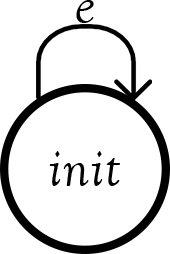
\includegraphics{null}\end{center}
  \item for \(\epsilon\), we have \(M = (\{init\},\ \Sigma^e,\ \delta,\ init,\ \{init\})\) and graphically \begin{center}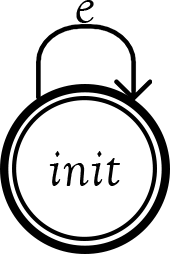
\includegraphics{epsilon}\end{center}
  \item for \(a\), we have \(M = (\{init, accept\},\ \Sigma^e,\ \delta,\ init,\ \{accept\})\) and graphically \begin{center}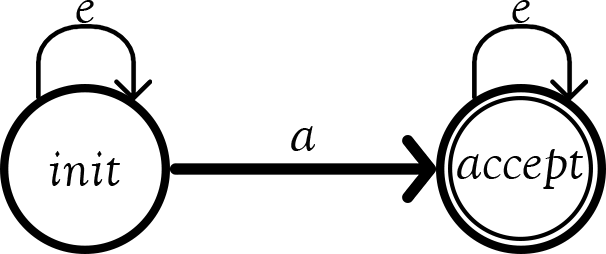
\includegraphics{singleton}\end{center}
  \item if \(N_1 = (Q_1,\ \delta_1,\ q_{01},\ F_1)\) and \(N_2 =
    (Q_2,\ \delta_2,\ q_{02},\ F_2)\) are \(\epsilon\)-NFAs translated from the
    regular expressions \(e_1\) and \(e_2\) respectively, then
    \begin{enumerate}
      \item for \((e_1\ |\ e_2)\), we have \(M = (\{init\} \cup Q_1
        \cup Q_2,\ \Sigma^e,\ \delta,\ init,\ F_1 \cup F_2)\) and
        graphically \begin{center}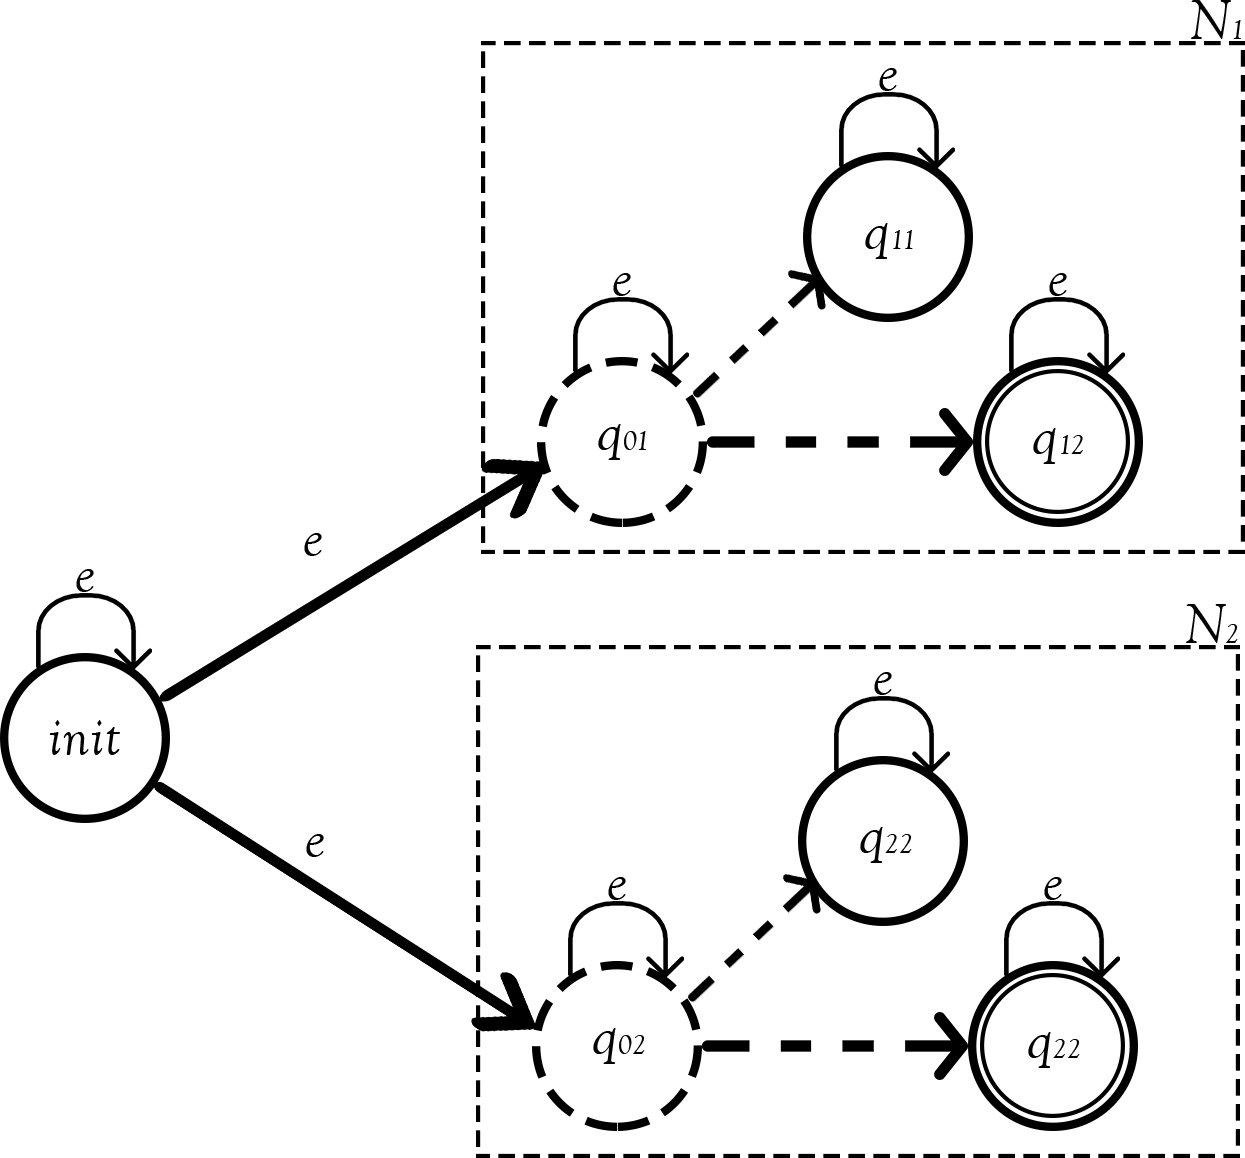
\includegraphics{union}\end{center}
      \item for \(e_{1}\cdot e_{2}\), we have \(M = (Q_1 \cup \{mid\}
        \cup Q_2,\ \Sigma^e,\ \delta,\ init,\ F_2)\) and graphically \begin{center}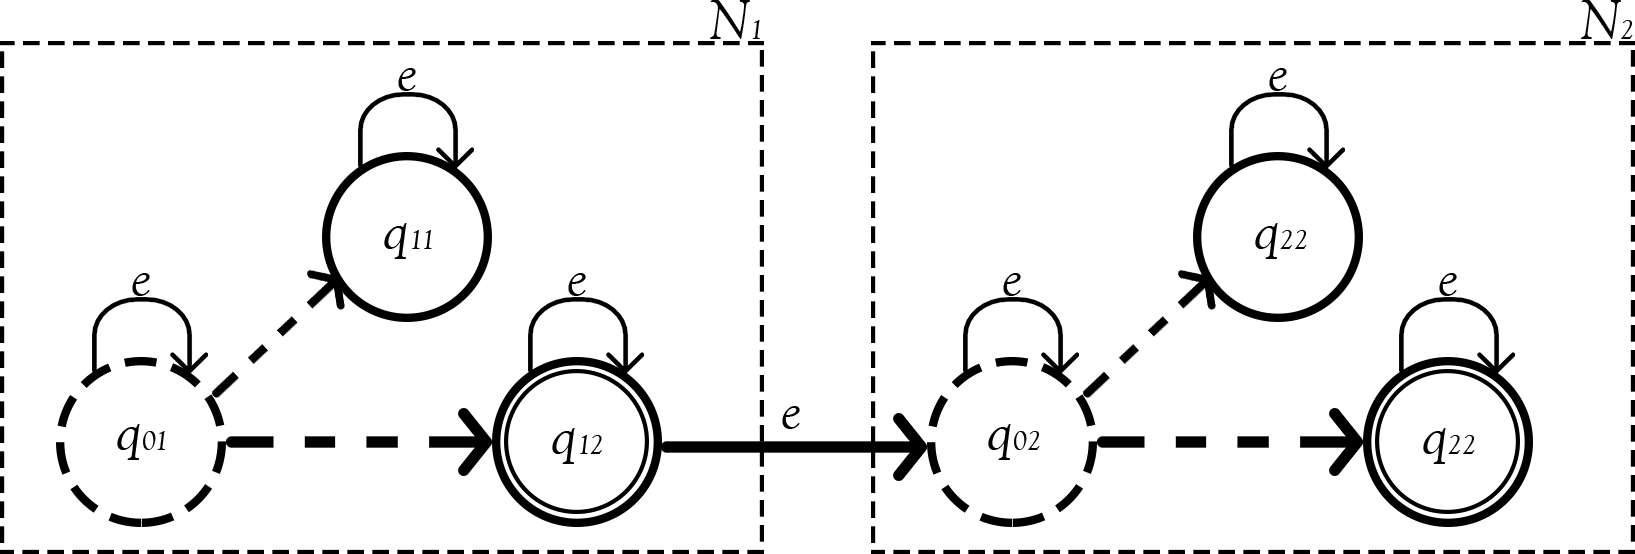
\includegraphics{concat}\end{center}
      \item for \(e_{1}^{\ *}\), we have \(M = (\{init\} \cup Q_1,\
        \Sigma^e,\ \delta,\ init,\ \{init\} \cup F_1)\) and
        graphically \begin{center}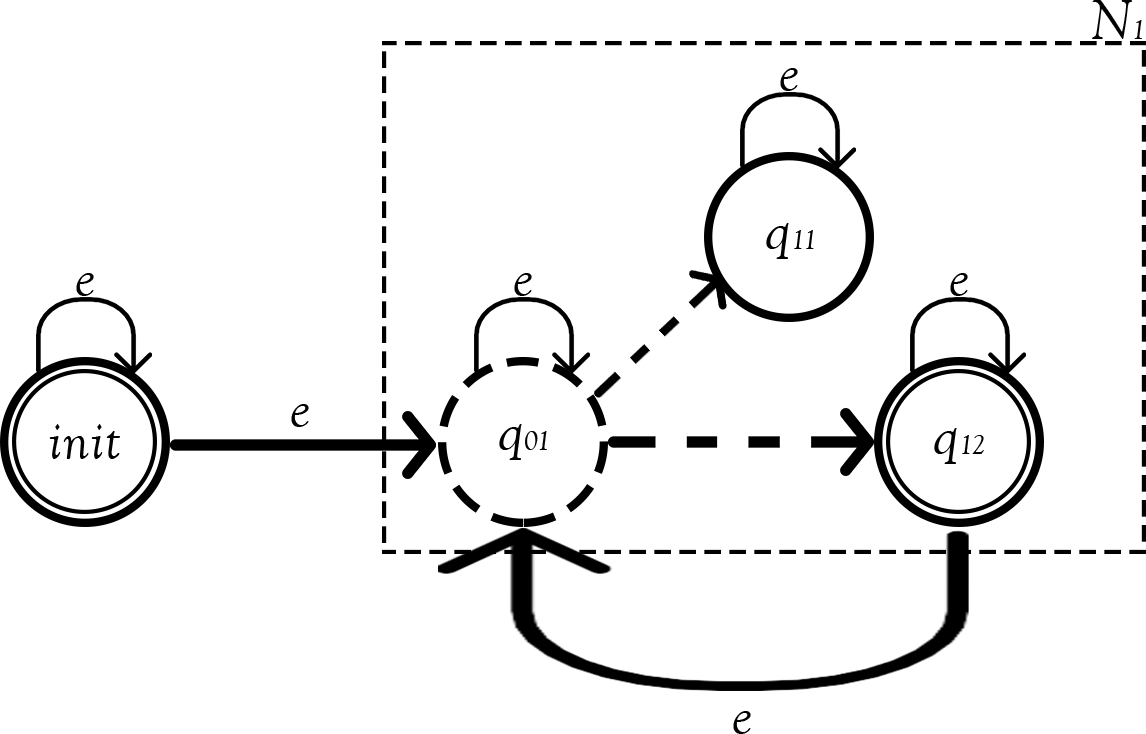
\includegraphics{star}\end{center}
     \end{enumerate}
\end{enumerate}


\paragraph{Theorem 1.1} For any given regular expression, the language accepted by it
is equal to the language accepted by its translated
\(\epsilon\)-NFA using Thompson's Construction. 

\paragraph{Proof 1.1} In order to prove \textbf{Theorem 1.1}, we have
to prove that for any regular expression \(e\), \(L(e) \subseteq
L(translated\ \epsilon\)-\(NFA)\) and \(L(e) \supseteq L(translated\
\epsilon\)-\(NFA)\).

\subsection{Non-deterministic Finite Automata}

\subsection{Removing \(\epsilon\)-transitions}

\subsection{Deterministic Finite Automata}

\subsection{Powerset Construction}

\subsection{Myhill-Nerode Theorem}

\section{Evaluation}
How easy/difficult to write proofs in Agda, compare to proofs written
in paper.

\section{Conclusion}
(?)

\section{References}
Aho, A. and Ullman, J. (1972). The Theory of Parsing, Translation and Compiling. Volume I: Parsing. United States of America: Prentice-Hall, Inc.

\section{Appendix}
Agda Code?

\end{document}